% Options for packages loaded elsewhere
\PassOptionsToPackage{unicode}{hyperref}
\PassOptionsToPackage{hyphens}{url}
%
\documentclass[
]{article}
\title{Informe HDT1}
\author{Marco Ramirez 19588-Alfredo Queza, Estuardo Hernandez}
\date{04/4/2022}

\usepackage{amsmath,amssymb}
\usepackage{lmodern}
\usepackage{iftex}
\ifPDFTeX
  \usepackage[T1]{fontenc}
  \usepackage[utf8]{inputenc}
  \usepackage{textcomp} % provide euro and other symbols
\else % if luatex or xetex
  \usepackage{unicode-math}
  \defaultfontfeatures{Scale=MatchLowercase}
  \defaultfontfeatures[\rmfamily]{Ligatures=TeX,Scale=1}
\fi
% Use upquote if available, for straight quotes in verbatim environments
\IfFileExists{upquote.sty}{\usepackage{upquote}}{}
\IfFileExists{microtype.sty}{% use microtype if available
  \usepackage[]{microtype}
  \UseMicrotypeSet[protrusion]{basicmath} % disable protrusion for tt fonts
}{}
\makeatletter
\@ifundefined{KOMAClassName}{% if non-KOMA class
  \IfFileExists{parskip.sty}{%
    \usepackage{parskip}
  }{% else
    \setlength{\parindent}{0pt}
    \setlength{\parskip}{6pt plus 2pt minus 1pt}}
}{% if KOMA class
  \KOMAoptions{parskip=half}}
\makeatother
\usepackage{xcolor}
\IfFileExists{xurl.sty}{\usepackage{xurl}}{} % add URL line breaks if available
\IfFileExists{bookmark.sty}{\usepackage{bookmark}}{\usepackage{hyperref}}
\hypersetup{
  pdftitle={Informe HDT1},
  pdfauthor={Marco Ramirez 19588-Alfredo Queza, Estuardo Hernandez},
  hidelinks,
  pdfcreator={LaTeX via pandoc}}
\urlstyle{same} % disable monospaced font for URLs
\usepackage[margin=1in]{geometry}
\usepackage{color}
\usepackage{fancyvrb}
\newcommand{\VerbBar}{|}
\newcommand{\VERB}{\Verb[commandchars=\\\{\}]}
\DefineVerbatimEnvironment{Highlighting}{Verbatim}{commandchars=\\\{\}}
% Add ',fontsize=\small' for more characters per line
\usepackage{framed}
\definecolor{shadecolor}{RGB}{248,248,248}
\newenvironment{Shaded}{\begin{snugshade}}{\end{snugshade}}
\newcommand{\AlertTok}[1]{\textcolor[rgb]{0.94,0.16,0.16}{#1}}
\newcommand{\AnnotationTok}[1]{\textcolor[rgb]{0.56,0.35,0.01}{\textbf{\textit{#1}}}}
\newcommand{\AttributeTok}[1]{\textcolor[rgb]{0.77,0.63,0.00}{#1}}
\newcommand{\BaseNTok}[1]{\textcolor[rgb]{0.00,0.00,0.81}{#1}}
\newcommand{\BuiltInTok}[1]{#1}
\newcommand{\CharTok}[1]{\textcolor[rgb]{0.31,0.60,0.02}{#1}}
\newcommand{\CommentTok}[1]{\textcolor[rgb]{0.56,0.35,0.01}{\textit{#1}}}
\newcommand{\CommentVarTok}[1]{\textcolor[rgb]{0.56,0.35,0.01}{\textbf{\textit{#1}}}}
\newcommand{\ConstantTok}[1]{\textcolor[rgb]{0.00,0.00,0.00}{#1}}
\newcommand{\ControlFlowTok}[1]{\textcolor[rgb]{0.13,0.29,0.53}{\textbf{#1}}}
\newcommand{\DataTypeTok}[1]{\textcolor[rgb]{0.13,0.29,0.53}{#1}}
\newcommand{\DecValTok}[1]{\textcolor[rgb]{0.00,0.00,0.81}{#1}}
\newcommand{\DocumentationTok}[1]{\textcolor[rgb]{0.56,0.35,0.01}{\textbf{\textit{#1}}}}
\newcommand{\ErrorTok}[1]{\textcolor[rgb]{0.64,0.00,0.00}{\textbf{#1}}}
\newcommand{\ExtensionTok}[1]{#1}
\newcommand{\FloatTok}[1]{\textcolor[rgb]{0.00,0.00,0.81}{#1}}
\newcommand{\FunctionTok}[1]{\textcolor[rgb]{0.00,0.00,0.00}{#1}}
\newcommand{\ImportTok}[1]{#1}
\newcommand{\InformationTok}[1]{\textcolor[rgb]{0.56,0.35,0.01}{\textbf{\textit{#1}}}}
\newcommand{\KeywordTok}[1]{\textcolor[rgb]{0.13,0.29,0.53}{\textbf{#1}}}
\newcommand{\NormalTok}[1]{#1}
\newcommand{\OperatorTok}[1]{\textcolor[rgb]{0.81,0.36,0.00}{\textbf{#1}}}
\newcommand{\OtherTok}[1]{\textcolor[rgb]{0.56,0.35,0.01}{#1}}
\newcommand{\PreprocessorTok}[1]{\textcolor[rgb]{0.56,0.35,0.01}{\textit{#1}}}
\newcommand{\RegionMarkerTok}[1]{#1}
\newcommand{\SpecialCharTok}[1]{\textcolor[rgb]{0.00,0.00,0.00}{#1}}
\newcommand{\SpecialStringTok}[1]{\textcolor[rgb]{0.31,0.60,0.02}{#1}}
\newcommand{\StringTok}[1]{\textcolor[rgb]{0.31,0.60,0.02}{#1}}
\newcommand{\VariableTok}[1]{\textcolor[rgb]{0.00,0.00,0.00}{#1}}
\newcommand{\VerbatimStringTok}[1]{\textcolor[rgb]{0.31,0.60,0.02}{#1}}
\newcommand{\WarningTok}[1]{\textcolor[rgb]{0.56,0.35,0.01}{\textbf{\textit{#1}}}}
\usepackage{graphicx}
\makeatletter
\def\maxwidth{\ifdim\Gin@nat@width>\linewidth\linewidth\else\Gin@nat@width\fi}
\def\maxheight{\ifdim\Gin@nat@height>\textheight\textheight\else\Gin@nat@height\fi}
\makeatother
% Scale images if necessary, so that they will not overflow the page
% margins by default, and it is still possible to overwrite the defaults
% using explicit options in \includegraphics[width, height, ...]{}
\setkeys{Gin}{width=\maxwidth,height=\maxheight,keepaspectratio}
% Set default figure placement to htbp
\makeatletter
\def\fps@figure{htbp}
\makeatother
\setlength{\emergencystretch}{3em} % prevent overfull lines
\providecommand{\tightlist}{%
  \setlength{\itemsep}{0pt}\setlength{\parskip}{0pt}}
\setcounter{secnumdepth}{-\maxdimen} % remove section numbering
\ifLuaTeX
  \usepackage{selnolig}  % disable illegal ligatures
\fi

\begin{document}
\maketitle

\hypertarget{hoja-de-trabajo-1-analisis-exploratorio}{%
\section{Hoja de Trabajo 1: Analisis
exploratorio}\label{hoja-de-trabajo-1-analisis-exploratorio}}

El objetivo de esta hoja de trabajo era realizar un analisis
exploratorio a la base de datos de peliculas, extraido de IMDB. Es base
cuenta con 10000 filas y con 27 de columnas.

\hypertarget{haga-una-exploraciuxf3n-ruxe1pida-de-sus-datos-para-eso-haga-un-resumen-de-su-conjunto-de-datos.}{%
\subsubsection{1. Haga una exploración rápida de sus datos, para eso
haga un resumen de su conjunto de
datos.}\label{haga-una-exploraciuxf3n-ruxe1pida-de-sus-datos-para-eso-haga-un-resumen-de-su-conjunto-de-datos.}}

\begin{Shaded}
\begin{Highlighting}[]
\FunctionTok{summary}\NormalTok{(datos)}
\end{Highlighting}
\end{Shaded}

\begin{verbatim}
##        id             budget             genres            homePage        
##  Min.   :     5   Min.   :        0   Length:10000       Length:10000      
##  1st Qu.: 12286   1st Qu.:        0   Class :character   Class :character  
##  Median :152558   Median :   500000   Mode  :character   Mode  :character  
##  Mean   :249877   Mean   : 18551632                                        
##  3rd Qu.:452022   3rd Qu.: 20000000                                        
##  Max.   :922260   Max.   :380000000                                        
##  productionCompany  productionCompanyCountry productionCountry 
##  Length:10000       Length:10000             Length:10000      
##  Class :character   Class :character         Class :character  
##  Mode  :character   Mode  :character         Mode  :character  
##                                                                
##                                                                
##                                                                
##     revenue             runtime        video           director        
##  Min.   :0.000e+00   Min.   :  0.0   Mode :logical   Length:10000      
##  1st Qu.:0.000e+00   1st Qu.: 90.0   FALSE:9430      Class :character  
##  Median :1.631e+05   Median :100.0   TRUE :84        Mode  :character  
##  Mean   :5.674e+07   Mean   :100.3   NA's :486                         
##  3rd Qu.:4.480e+07   3rd Qu.:113.0                                     
##  Max.   :2.847e+09   Max.   :750.0                                     
##     actors          actorsPopularity   actorsCharacter    originalTitle     
##  Length:10000       Length:10000       Length:10000       Length:10000      
##  Class :character   Class :character   Class :character   Class :character  
##  Mode  :character   Mode  :character   Mode  :character   Mode  :character  
##                                                                             
##                                                                             
##                                                                             
##     title           originalLanguage     popularity        releaseDate       
##  Length:10000       Length:10000       Min.   :    4.258   Length:10000      
##  Class :character   Class :character   1st Qu.:   14.578   Class :character  
##  Mode  :character   Mode  :character   Median :   21.906   Mode  :character  
##                                        Mean   :   51.394                     
##                                        3rd Qu.:   40.654                     
##                                        Max.   :11474.647                     
##     voteAvg         voteCount      genresAmount    productionCoAmount
##  Min.   : 1.300   Min.   :    1   Min.   : 0.000   Min.   : 0.000    
##  1st Qu.: 5.900   1st Qu.:  120   1st Qu.: 2.000   1st Qu.: 2.000    
##  Median : 6.500   Median :  415   Median : 3.000   Median : 3.000    
##  Mean   : 6.483   Mean   : 1342   Mean   : 2.596   Mean   : 3.171    
##  3rd Qu.: 7.200   3rd Qu.: 1316   3rd Qu.: 3.000   3rd Qu.: 4.000    
##  Max.   :10.000   Max.   :30788   Max.   :16.000   Max.   :89.000    
##  productionCountriesAmount  actorsAmount    castWomenAmount   
##  Min.   :  0.000           Min.   :     0   Length:10000      
##  1st Qu.:  1.000           1st Qu.:    13   Class :character  
##  Median :  1.000           Median :    21   Mode  :character  
##  Mean   :  1.751           Mean   :  2148                     
##  3rd Qu.:  2.000           3rd Qu.:    36                     
##  Max.   :155.000           Max.   :919590                     
##  castMenAmount     
##  Length:10000      
##  Class :character  
##  Mode  :character  
##                    
##                    
## 
\end{verbatim}

\hypertarget{diga-el-tipo-de-cada-una-de-las-variables-cualitativa-ordinal-o-nominal-cuantitativa-continua-cuantitativa-discreta}{%
\subsubsection{2. Diga el tipo de cada una de las variables (cualitativa
ordinal o nominal, cuantitativa continua, cuantitativa
discreta)}\label{diga-el-tipo-de-cada-una-de-las-variables-cualitativa-ordinal-o-nominal-cuantitativa-continua-cuantitativa-discreta}}

\begin{figure}
\centering
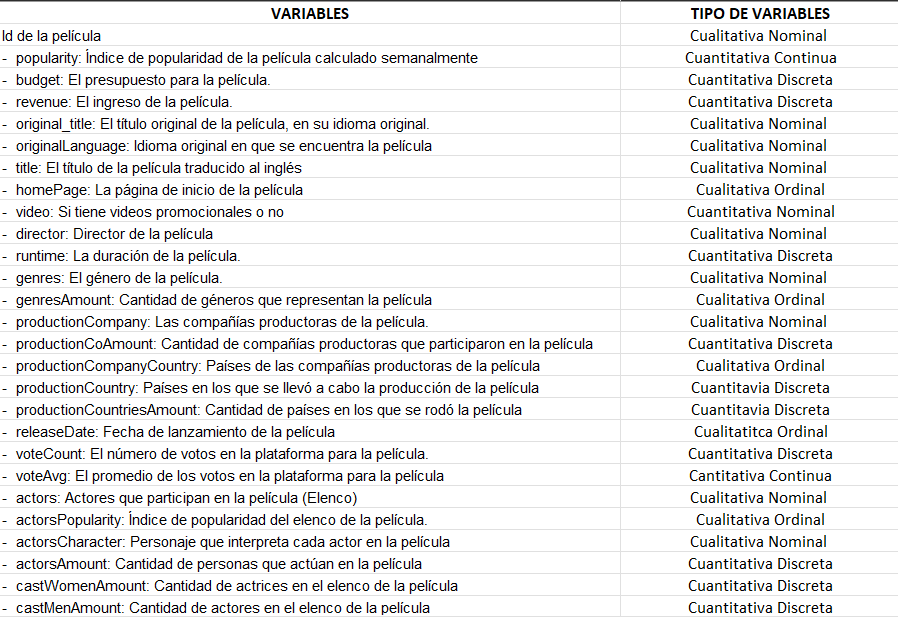
\includegraphics{/Users/MAQUITO/Desktop/UVG/UVG S7/Mineria de datos/HDT1/HDT1_F/HT1_Mineria/Ejercicio2.png}
\caption{Caption for the picture.}
\end{figure}

\hypertarget{investigue-si-las-variables-cuantitativas-siguen-una-distribuciuxf3n-normal-y-haga-una-tabla-de-frecuencias-de-las-variables-cualitativas.-explique-todos-los-resultados.}{%
\subsubsection{3. Investigue si las variables cuantitativas siguen una
distribución normal y haga una tabla de frecuencias de las variables
cualitativas. Explique todos los
resultados.}\label{investigue-si-las-variables-cuantitativas-siguen-una-distribuciuxf3n-normal-y-haga-una-tabla-de-frecuencias-de-las-variables-cualitativas.-explique-todos-los-resultados.}}

\hypertarget{responda-las-siguientes-preguntas}{%
\subsubsection{4. Responda las siguientes
preguntas}\label{responda-las-siguientes-preguntas}}

\hypertarget{cuuxe1les-son-las-10-peluxedculas-que-contaron-con-muxe1s-presupuesto}{%
\subsubsection{4.1. ¿Cuáles son las 10 películas que contaron con más
presupuesto?}\label{cuuxe1les-son-las-10-peluxedculas-que-contaron-con-muxe1s-presupuesto}}

\begin{Shaded}
\begin{Highlighting}[]
\NormalTok{pregunta1}
\end{Highlighting}
\end{Shaded}

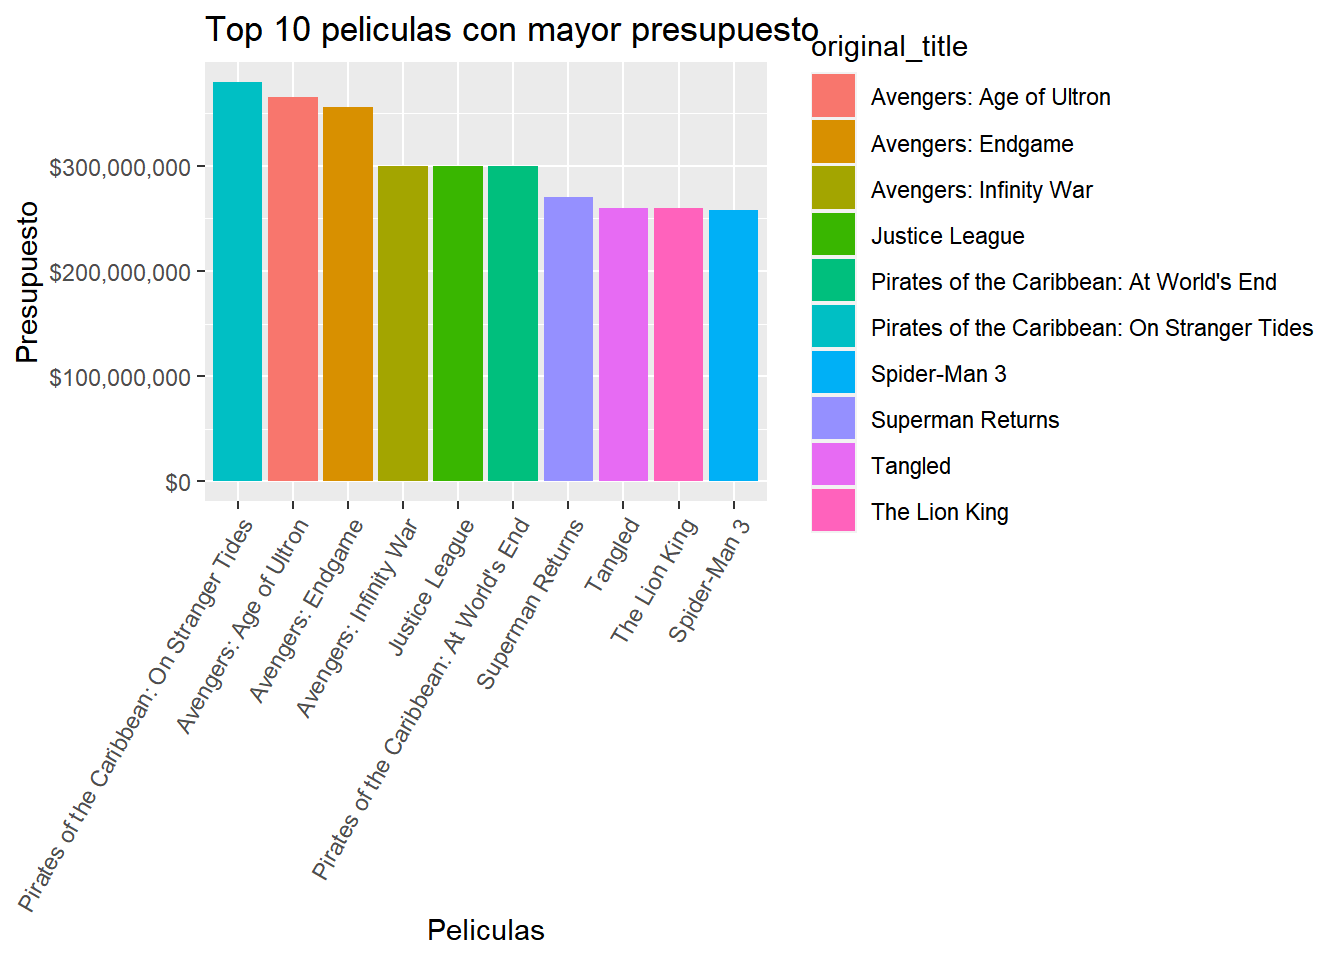
\includegraphics{InformeHoja1_files/figure-latex/unnamed-chunk-4-1.pdf}

\n

\hypertarget{como-se-observa-en-la-grafica-anterior-las-10-peliculas-con-mayor-presupuesto-son}{%
\paragraph{\texorpdfstring{Como se observa en la grafica anterior las 10
peliculas con mayor presupuesto
son:\n}{Como se observa en la grafica anterior las 10 peliculas con mayor presupuesto son:}}\label{como-se-observa-en-la-grafica-anterior-las-10-peliculas-con-mayor-presupuesto-son}}

\begin{enumerate}
\def\labelenumi{\arabic{enumi}.}
\tightlist
\item
  \textbf{Pirates of the Caribbean: On Stranger Tides} con un
  presupuesto de \textbf{380000000} dolares.
\item
  \textbf{Avengers: Age of Ultron} con un presupuesto de
  \textbf{365000000} dolares.
\item
  \textbf{Avengers: Endgame} con un presupuesto de \textbf{356000000}
  dolares.
\item
  \textbf{Pirates of the Caribbean: At World's End} con un presupuesto
  de \textbf{300000000} dolares.
\item
  \textbf{Justice League} con un presupuesto de \textbf{300000000}
  dolares.
\item
  \textbf{Avengers: Infinity War} con un presupuesto de
  \textbf{300000000} dolares.
\item
  \textbf{Superman Returns} con un presupuesto de \textbf{270000000}
  dolares.
\item
  \textbf{Tangled} con un presupuesto de \textbf{260000000} dolares.
\item
  \textbf{The Lion King} con un presupuesto de \textbf{260000000}
  dolares.
\item
  \textbf{Spider-Man 3} con un presupuesto de \textbf{258000000}
  dolares.
\end{enumerate}

\hypertarget{cuuxe1les-son-las-10-peluxedculas-que-muxe1s-ingresos-tuvieron}{%
\subsubsection{4.2. ¿Cuáles son las 10 películas que más ingresos
tuvieron?}\label{cuuxe1les-son-las-10-peluxedculas-que-muxe1s-ingresos-tuvieron}}

\hypertarget{cuuxe1l-es-la-peluxedcula-que-muxe1s-votos-tuvo}{%
\subsubsection{4.3. ¿Cuál es la película que más votos
tuvo?}\label{cuuxe1l-es-la-peluxedcula-que-muxe1s-votos-tuvo}}

\begin{Shaded}
\begin{Highlighting}[]
\NormalTok{pregunta4}\FloatTok{.3}
\end{Highlighting}
\end{Shaded}

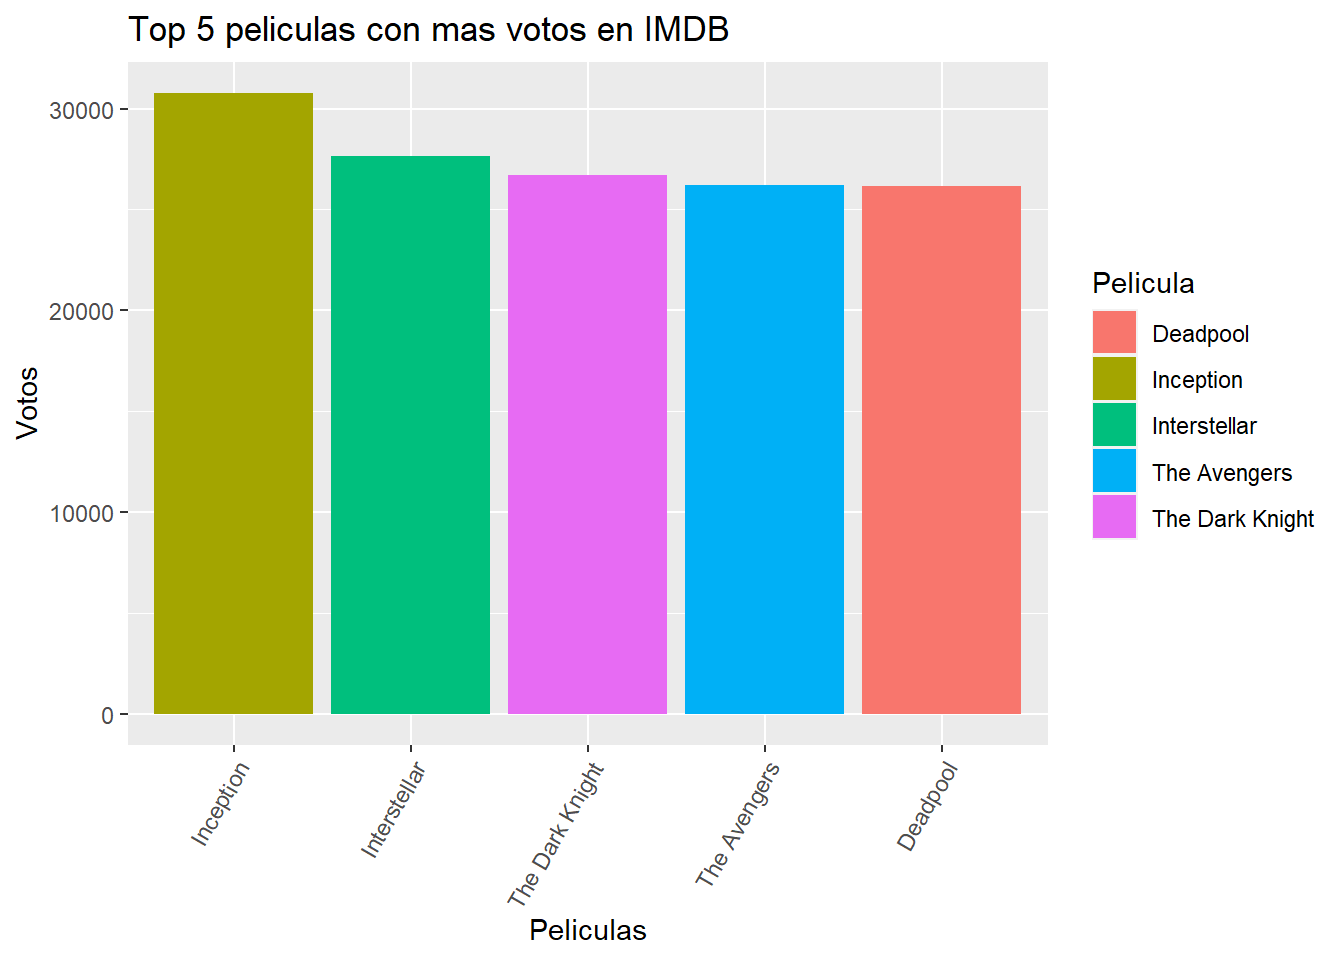
\includegraphics{InformeHoja1_files/figure-latex/unnamed-chunk-6-1.pdf}

\hypertarget{como-se-observa-en-la-grafica-anterior-las-10-peliculas-con-mayor-presupuesto-son-1}{%
\paragraph{\texorpdfstring{Como se observa en la grafica anterior las 10
peliculas con mayor presupuesto
son:\n}{Como se observa en la grafica anterior las 10 peliculas con mayor presupuesto son:}}\label{como-se-observa-en-la-grafica-anterior-las-10-peliculas-con-mayor-presupuesto-son-1}}

\begin{enumerate}
\def\labelenumi{\arabic{enumi}.}
\tightlist
\item
  \textbf{Inception} con \textbf{30788} de votos.
\item
  \textbf{Interstellar} con \textbf{27644} de votos.
\item
  \textbf{The Dark Knight} con \textbf{26690} de votos.
\item
  \textbf{The Avengers} con \textbf{26215} de votos.
\item
  \textbf{Deadpool} con \textbf{26178} de votos.
\end{enumerate}

\hypertarget{cuuxe1l-es-la-peor-peluxedcula-de-acuerdo-a-los-votos-de-todos-los-usuarios}{%
\subsubsection{4.4. ¿Cuál es la peor película de acuerdo a los votos de
todos los
usuarios?}\label{cuuxe1l-es-la-peor-peluxedcula-de-acuerdo-a-los-votos-de-todos-los-usuarios}}

\hypertarget{cuuxe1ntas-peluxedculas-se-hicieron-en-cada-auxf1o-en-quuxe9-auxf1o-se-hicieron-muxe1s-peluxedculas-haga-un-gruxe1fico-de-barras}{%
\subsubsection{4.5. ¿Cuántas películas se hicieron en cada año? ¿En qué
año se hicieron más películas? Haga un gráfico de
barras}\label{cuuxe1ntas-peluxedculas-se-hicieron-en-cada-auxf1o-en-quuxe9-auxf1o-se-hicieron-muxe1s-peluxedculas-haga-un-gruxe1fico-de-barras}}

\hypertarget{cuuxe1l-es-el-guxe9nero-principal-de-las-20-peluxedculas-muxe1s-recientes-cuuxe1l-es-el-guxe9nero-principal-que-predomina-en-el-conjunto-de-datos-represuxe9ntelo-usando-un-gruxe1fico}{%
\subsubsection{4.6. ¿Cuál es el género principal de las 20 películas más
recientes? ¿Cuál es el género principal que predomina en el conjunto de
datos? Represéntelo usando un
gráfico}\label{cuuxe1l-es-el-guxe9nero-principal-de-las-20-peluxedculas-muxe1s-recientes-cuuxe1l-es-el-guxe9nero-principal-que-predomina-en-el-conjunto-de-datos-represuxe9ntelo-usando-un-gruxe1fico}}

\begin{Shaded}
\begin{Highlighting}[]
\NormalTok{pregunta4}\FloatTok{.6}
\end{Highlighting}
\end{Shaded}

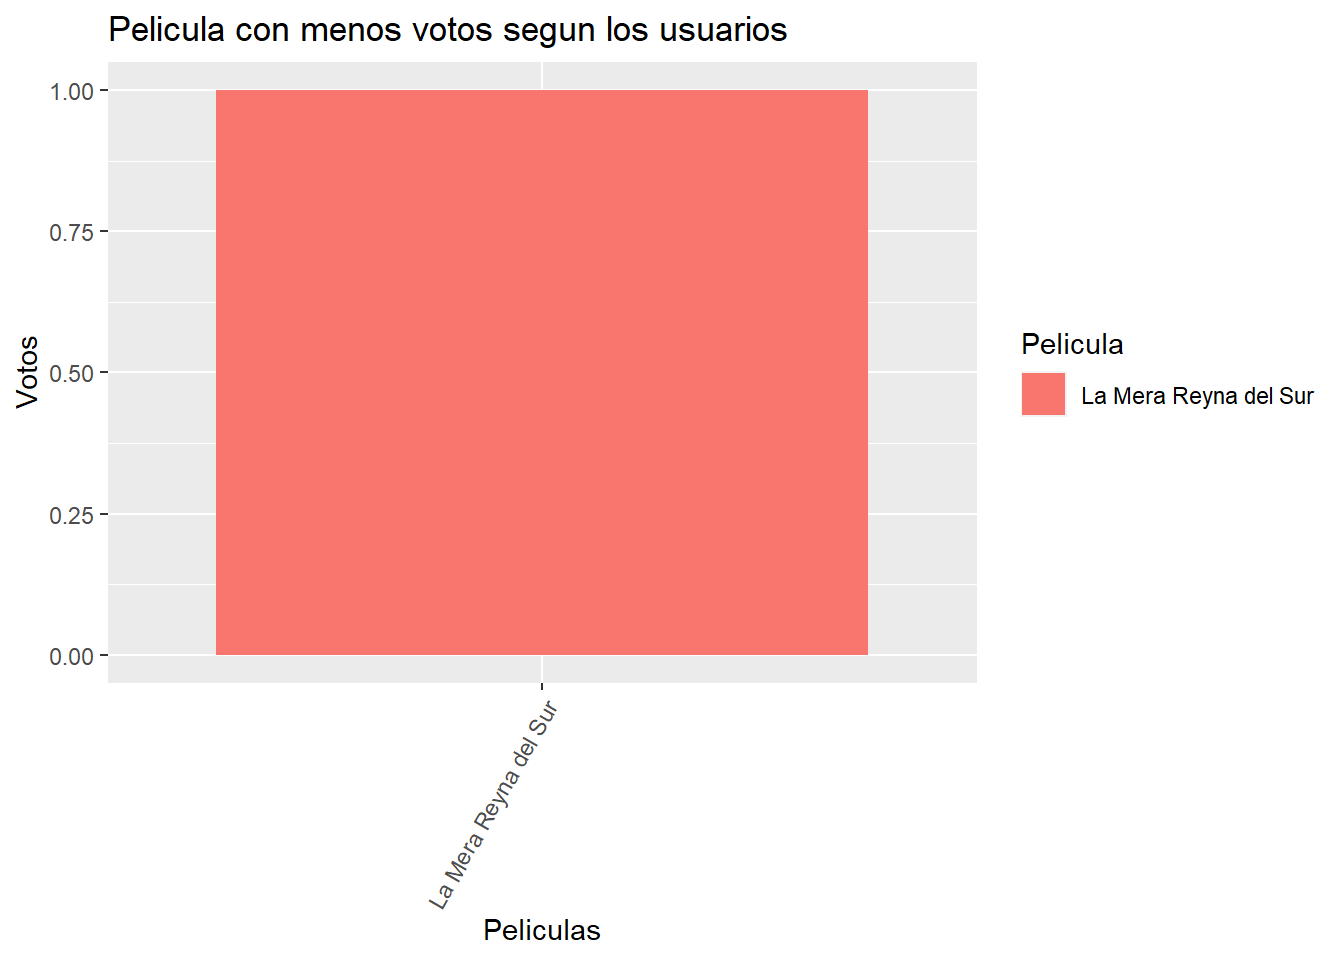
\includegraphics{InformeHoja1_files/figure-latex/unnamed-chunk-8-1.pdf}

\hypertarget{como-se-observa-en-la-grafica-anterior-los-generos-principales-de-las-20-peliculas-mas-recientes-son}{%
\paragraph{Como se observa en la grafica anterior los generos
principales de las 20 peliculas mas recientes
son:}\label{como-se-observa-en-la-grafica-anterior-los-generos-principales-de-las-20-peliculas-mas-recientes-son}}

\begin{enumerate}
\def\labelenumi{\arabic{enumi}.}
\tightlist
\item
  \textbf{Comedy} repitiendose \textbf{3} veces.
\item
  \textbf{Drama} repitiendose \textbf{2} veces.
\item
  \textbf{El resto de generos} repitiendose \textbf{1} veces.
\end{enumerate}

\hypertarget{es-posible-que-la-cantidad-de-hombres-y-mujeres-en-el-reparto-influya-en-la-popularidad-y-los-ingresos-de-las-peluxedculas}{%
\subsubsection{4.9. ¿Es posible que la cantidad de hombres y mujeres en
el reparto influya en la popularidad y los ingresos de las
películas?}\label{es-posible-que-la-cantidad-de-hombres-y-mujeres-en-el-reparto-influya-en-la-popularidad-y-los-ingresos-de-las-peluxedculas}}

\begin{Shaded}
\begin{Highlighting}[]
\FunctionTok{pie}\NormalTok{(x, }\AttributeTok{labels=}\NormalTok{piepercent, }\AttributeTok{main =} \StringTok{"Porcentaje de ganancias de las peliculas cuando hay un sexo predominante"}\NormalTok{, }\AttributeTok{col =} \FunctionTok{rainbow}\NormalTok{(}\FunctionTok{length}\NormalTok{(x)))}
                \FunctionTok{legend}\NormalTok{(}\StringTok{"topright"}\NormalTok{, }\FunctionTok{c}\NormalTok{(}\StringTok{"Hombres"}\NormalTok{,}\StringTok{"Mujeres"}\NormalTok{), }\AttributeTok{cex =} \FloatTok{0.8}\NormalTok{,}
                       \AttributeTok{fill =} \FunctionTok{rainbow}\NormalTok{(}\FunctionTok{length}\NormalTok{(x)))}
\end{Highlighting}
\end{Shaded}

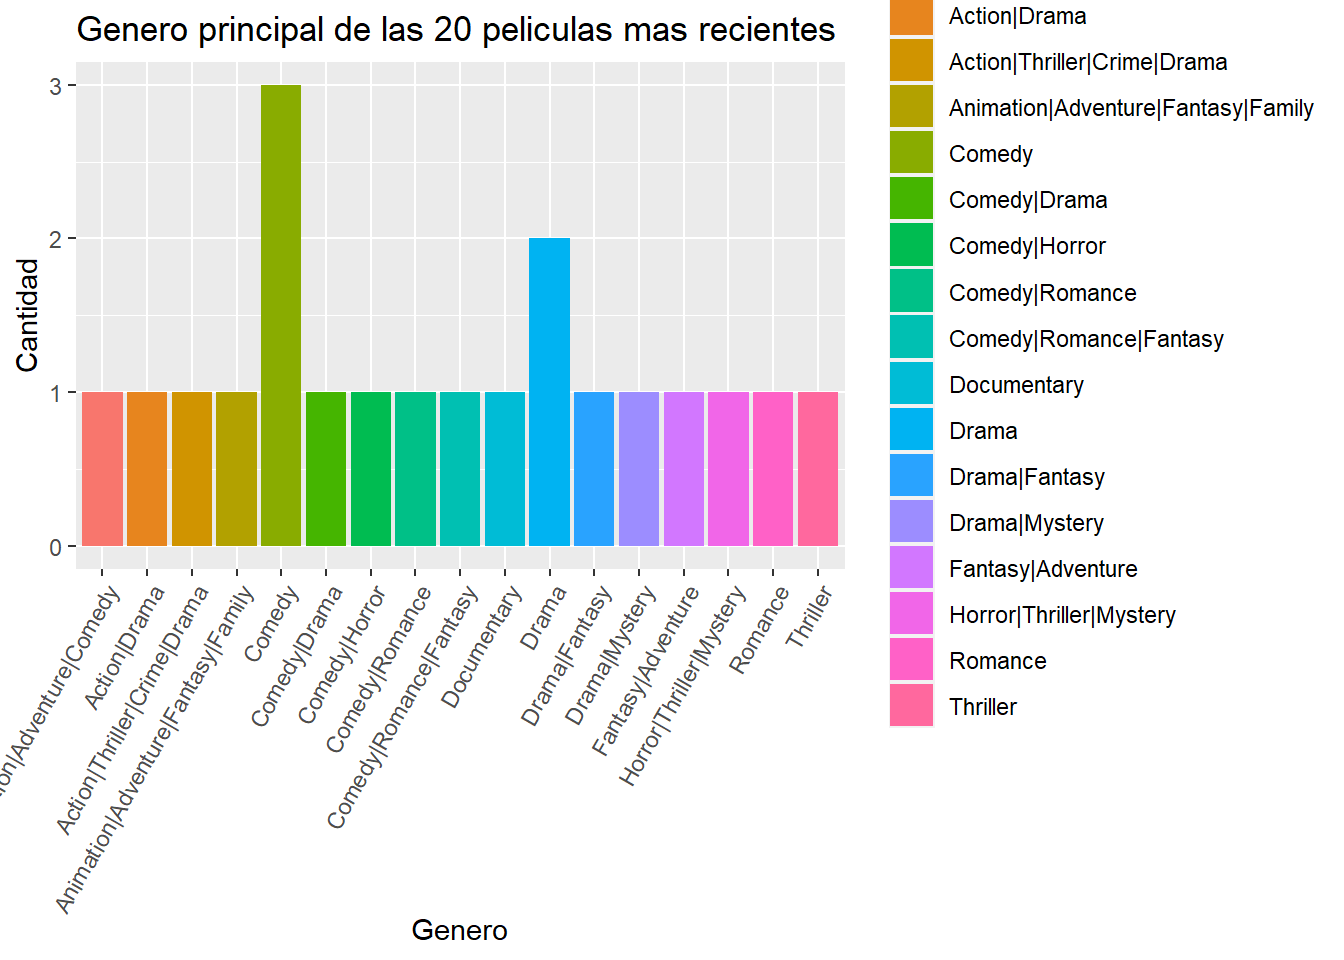
\includegraphics{InformeHoja1_files/figure-latex/unnamed-chunk-10-1.pdf}

Como se observa en la grafica, del 100\% de los ingresos de las
peliculas en la base de datos, se demuestra que el 91.4\% de los
ingresos se debe cuando hay mas actores que actrices.

\begin{Shaded}
\begin{Highlighting}[]
\FunctionTok{pie}\NormalTok{(xPopu, }\AttributeTok{labels=}\NormalTok{piepercentPopu, }\AttributeTok{main =} \StringTok{"Porcentaje de popularidad de las peliculas cuando hay un sexo predominante"}\NormalTok{, }\AttributeTok{col =} \FunctionTok{rainbow}\NormalTok{(}\FunctionTok{length}\NormalTok{(x)))}
\FunctionTok{legend}\NormalTok{(}\StringTok{"topright"}\NormalTok{, }\FunctionTok{c}\NormalTok{(}\StringTok{"Hombres"}\NormalTok{,}\StringTok{"Mujeres"}\NormalTok{), }\AttributeTok{cex =} \FloatTok{0.8}\NormalTok{,}
       \AttributeTok{fill =} \FunctionTok{rainbow}\NormalTok{(}\FunctionTok{length}\NormalTok{(xPopu)))}
\end{Highlighting}
\end{Shaded}

\includegraphics{InformeHoja1_files/figure-latex/unnamed-chunk-11-1.pdf}

Y como se ve en la grafica de pie, se observa que las peliculas con mas
hombres que mujeres otienen mayor popularidad. Sin embargo, estos
porcentajes son menores a diferencia de los porcentajes de ingresos.

\hypertarget{se-asocian-ciertos-meses-de-lanzamiento-con-mejores-ingresos}{%
\subsubsection{4.12. ¿Se asocian ciertos meses de lanzamiento con
mejores
ingresos?}\label{se-asocian-ciertos-meses-de-lanzamiento-con-mejores-ingresos}}

\begin{Shaded}
\begin{Highlighting}[]
\NormalTok{pregunta4}\FloatTok{.12}
\end{Highlighting}
\end{Shaded}

\includegraphics{InformeHoja1_files/figure-latex/unnamed-chunk-13-1.pdf}
Para la elaboracion de esta grafica fue necesario promediar el ingreso
de las peliculas respecto a su mes de lanzamiento, evidenciando que el
mes con mayor ingresos segun su fecha de lanzamiento es \textbf{Junio} ,
siguiendo \textbf{Mayo} y como tercer lugar a \textbf{Julio}.
Demostrando que el peor mes para lanzar una pelicual es
\textbf{Septiembre}

\hypertarget{a-quuxe9-guxe9nero-principal-pertenecen-las-peluxedculas-muxe1s-largas}{%
\subsubsection{4.15. ¿A qué género principal pertenecen las películas
más
largas?}\label{a-quuxe9-guxe9nero-principal-pertenecen-las-peluxedculas-muxe1s-largas}}

\begin{Shaded}
\begin{Highlighting}[]
\NormalTok{pregunta4}\FloatTok{.15}
\end{Highlighting}
\end{Shaded}

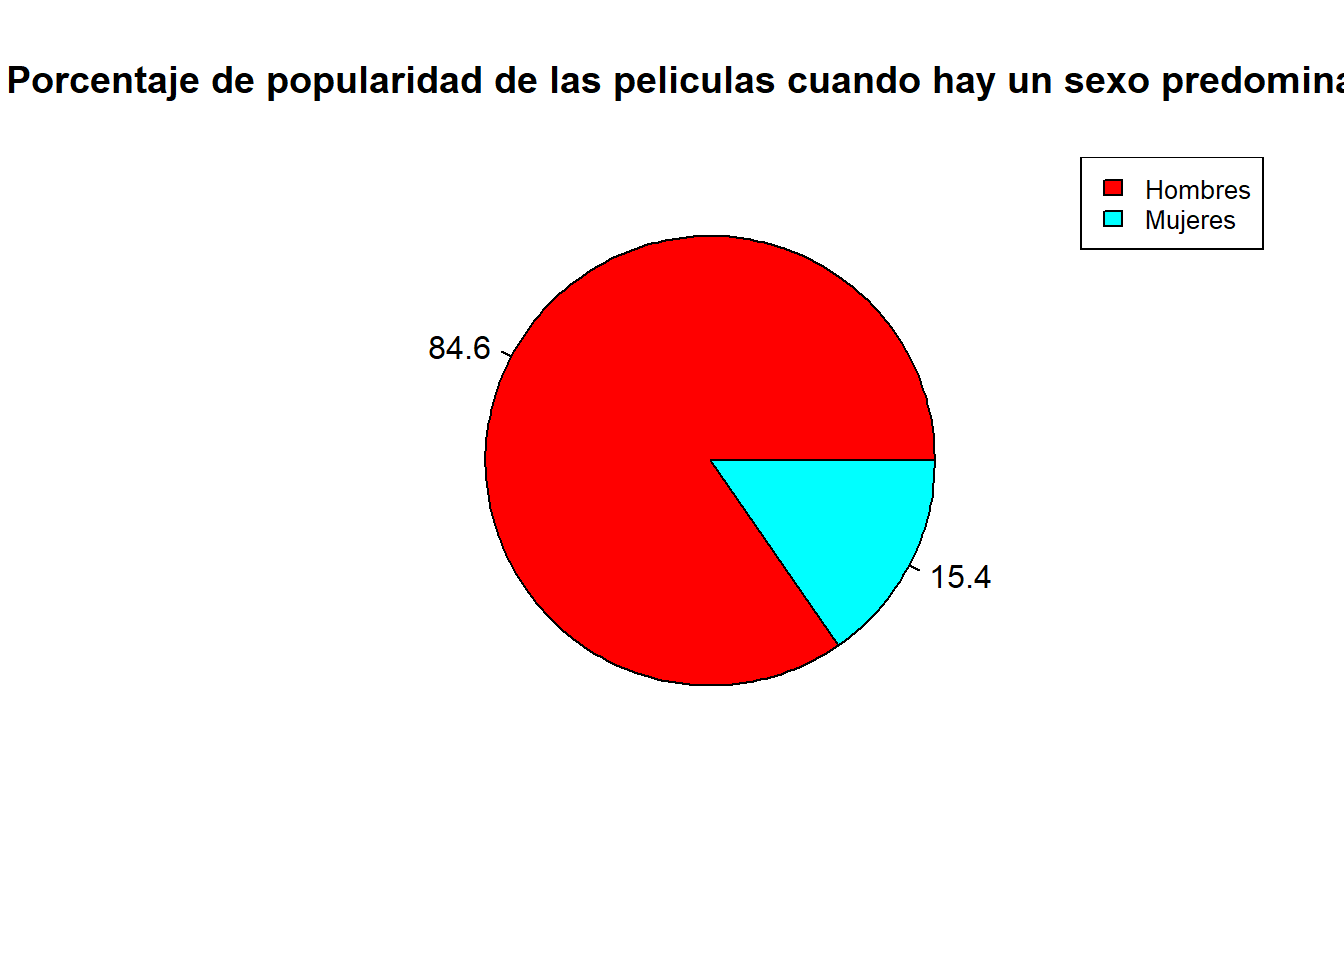
\includegraphics{InformeHoja1_files/figure-latex/unnamed-chunk-15-1.pdf}

Como se observa en la grafica anterior , las 5 peliculas con mayor
duracion y su respectivo genero fueron:

\begin{enumerate}
\def\labelenumi{\arabic{enumi}.}
\item
  \textbf{\textless U+30DD\textgreater\textless U+30CB\textgreater\textless U+30E7\textgreater\textless U+306F\textgreater\textless U+3053\textgreater\textless U+3046\textgreater\textless U+3057\textgreater\textless U+3066\textgreater\textless U+751F\textgreater\textless U+307E\textgreater\textless U+308C\textgreater\textless U+305F\textgreater{}
  \textless U+301C\textgreater{}
  \textless U+5BAE\textgreater\textless U+FA11\textgreater\textless U+99FF\textgreater\textless U+306E\textgreater\textless U+601D\textgreater\textless U+8003\textgreater\textless U+904E\textgreater\textless U+7A0B\textgreater{}
  \textless U+301C\textgreater{}} con una duracion de \textbf{750}
  minutos y su genero es \textbf{Documentary} (cabe mencionar que para
  fines estadisticos fue necesario cambiar el nombre de esta pelicula
  por ``Pelicula con mayor duracion'' esto debido que su nombre era
  demasiado largo para mostrar graficamente).
\item
  \textbf{Crystal Lake Memories: The Complete History of Friday the
  13th} con una duracion de \textbf{400} minutos y su genero es
  \textbf{Documentary}
\item
  \textbf{Napoléon} con una duracion de \textbf{333} minutos y su genero
  es \textbf{Drama\textbar History\textbar War}
\item
  \textbf{Novecento} con una duracion de \textbf{317} minutos y su
  genero es \textbf{Drama\textbar History}
\item
  \textbf{Cleopatra} con una duracion de \textbf{248} minutos y su
  genero es \textbf{Drama\textbar History\textbar Romance}
\item
  \textbf{Kill Bill: The Whole Bloody Affair} con una duracion de
  \textbf{247} minutos y su genero es
  \textbf{Action\textbar Crime\textbar Thriller}
\item
  \textbf{Hamlet} con una duracion de \textbf{242} minutos y su genero
  es \textbf{Drama}
\end{enumerate}

\end{document}
